\documentclass{beamer}
\usepackage[utf8]{inputenc}

\usetheme{Madrid}
\usecolortheme{default}
\usepackage{amsmath,amssymb,amsfonts,amsthm}
\usepackage{txfonts}
\usepackage{tkz-euclide}
\usepackage{listings}
\usepackage{adjustbox}
\usepackage{array}
\usepackage{tabularx}
\usepackage{gvv}
\usepackage{lmodern}
\usepackage{circuitikz}
\usepackage{tikz}
\usepackage{graphicx}

\setbeamertemplate{page number in head/foot}[totalframenumber]

\usepackage{tcolorbox}
\tcbuselibrary{minted,breakable,xparse,skins}



\definecolor{bg}{gray}{0.95}
\DeclareTCBListing{mintedbox}{O{}m!O{}}{%
  breakable=true,
  listing engine=minted,
  listing only,
  minted language=#2,
  minted style=default,
  minted options={%
    linenos,
    gobble=0,
    breaklines=true,
    breakafter=,,
    fontsize=\small,
    numbersep=8pt,
    #1},
  boxsep=0pt,
  left skip=0pt,
  right skip=0pt,
  left=25pt,
  right=0pt,
  top=3pt,
  bottom=3pt,
  arc=5pt,
  leftrule=0pt,
  rightrule=0pt,
  bottomrule=2pt,
  toprule=2pt,
  colback=bg,
  colframe=orange!70,
  enhanced,
  overlay={%
    \begin{tcbclipinterior}
    \fill[orange!20!white] (frame.south west) rectangle ([xshift=20pt]frame.north west);
    \end{tcbclipinterior}},
  #3,
}
\lstset{
    language=C,
    basicstyle=\ttfamily\small,
    keywordstyle=\color{blue},
    stringstyle=\color{orange},
    commentstyle=\color{green!60!black},
    numbers=left,
    numberstyle=\tiny\color{gray},
    breaklines=true,
    showstringspaces=false,
}
\begin{document}

\title 
{2.4.31}
\date{September 9,2025}


\author 
{Kishora Karthik-EE25BTECH11034}
\frame{\titlepage}
\begin{frame}{Question}
Check if the point $\vec{A}(2, 7)$ lies on the perpendicular bisector of line segment joining the points
$\vec{P}(6, 5)$ and $\vec{Q}(0, -4)$.\\\\
\end{frame}



\begin{frame}{ Solution}
The equation of the perpendicular bisector of PQ is\\
\begin{align}
    \brak{\vec{A}-\frac{\vec{P}+\vec{Q}}{2}}^\top\brak{\vec{P}-\vec{Q}}=0
\end{align}
The given points are,\\
\begin{align}
    \vec{A}=\myvec{2\\7}\\
    \vec{P}=\myvec{6\\5}\\
    \vec{Q}=\myvec{0\\-4}
\end{align}
\begin{align}
    \vec{P}-\vec{Q}=\myvec{6\\5}-\myvec{0\\-4}\\
\end{align}
\end{frame}

\begin{frame}{Solution}
   \begin{align}
        \vec{P}-\vec{Q}=\myvec{6\\9}
\end{align}
\begin{align}
    \frac{\vec{P}+\vec{Q}}{2}={\frac{\myvec{6\\5}+\myvec{0\\-4}}{2}}
\end{align}
\begin{align}
    \frac{\vec{P}+\vec{Q}}{2}={\frac{\myvec{6\\1}}{2}}\\
    \frac{\vec{P}+\vec{Q}}{2}=\myvec{3\\0.5}   
\end{align}
\begin{align}
    \vec{A}-\frac{\vec{P}+\vec{Q}}{2}=\myvec{2\\7}-\myvec{3\\0.5} 
\end{align}
\end{frame}
\begin{frame}{Solution}
\begin{align}
    \vec{A}-\frac{\vec{P}+\vec{Q}}{2}=\myvec{-1\\6.5}   
\end{align}
\begin{align}
    \brak{\vec{A}-\frac{\vec{P}+\vec{Q}}{2}}^\top\brak{\vec{P}-\vec{Q}}=\myvec{-1&6.5}\myvec{6\\9}
\end{align}
\begin{align}
    \brak{\vec{A}-\frac{\vec{P}+\vec{Q}}{2}}^\top\brak{\vec{P}-\vec{Q}}=(-1)(6)+(6.5)(9)
\end{align}
\begin{align}
    \brak{\vec{A}-\frac{\vec{P}+\vec{Q}}{2}}^\top\brak{\vec{P}-\vec{Q}}=52.5\neq0
\end{align}
The equation of perpendicular bisector is not satisfied.
Therefore, point $\vec{A}$ does not lie on the perpendicular bisector of line segment joining the points $\vec{P}$ and $\vec{Q}$.
\end{frame}
\begin{frame}{Plot}
    \centering
    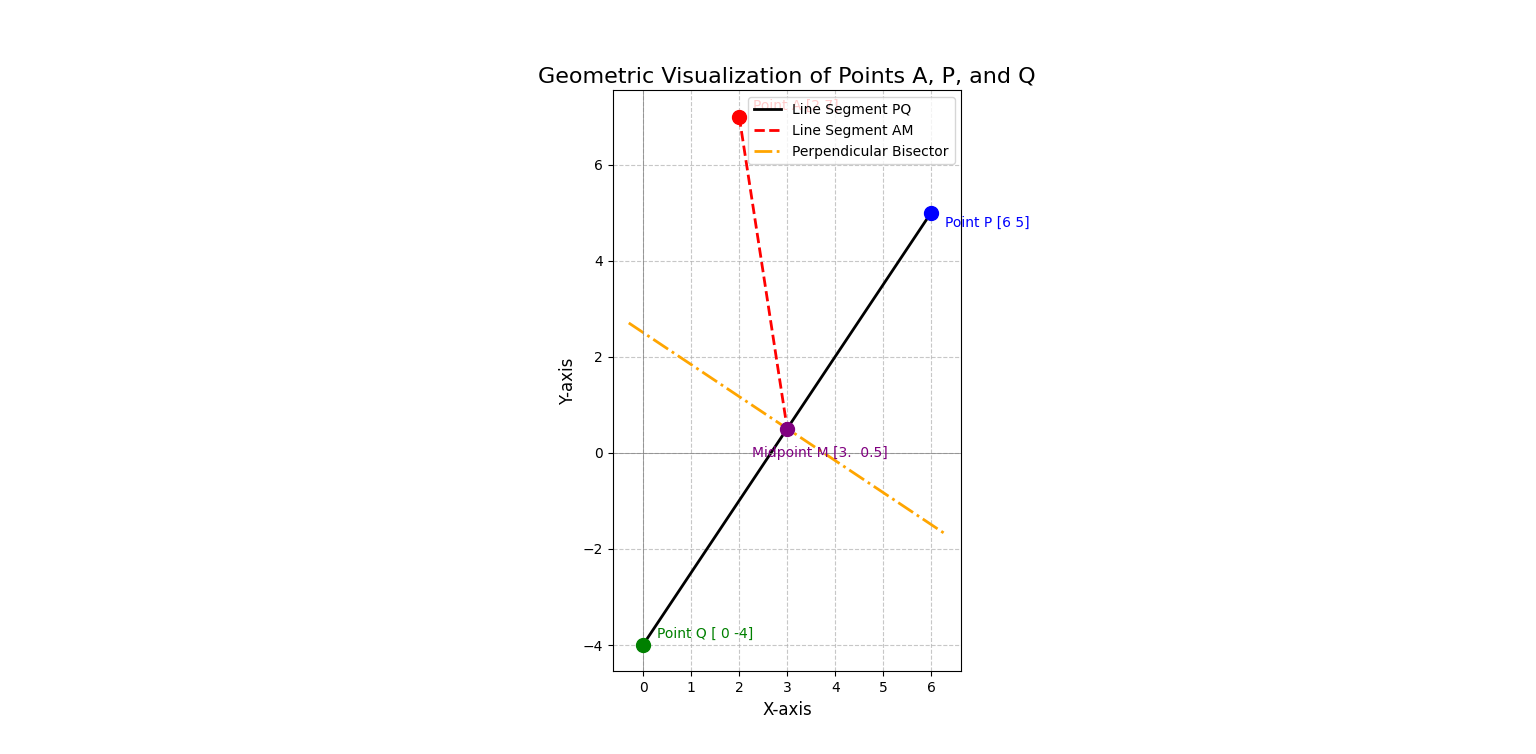
\includegraphics[width=\columnwidth, height=0.8\textheight, keepaspectratio]{figs/fig1.png} 
\end{frame}

\end{document}

